\chapter{Contribution}

Most important chapter of the thesis. Describes what the author contributes as research. Discusses intuition, motivation, describes and reasons about necessity of proposed elements. Defines theses based on reasonable assumptions. Discusses relevant aspects of contribution. Approximately 30 to 40 pages. Can be split into multiple chapters.
\\\\
Eine grundlegende Entscheidungen zu Beginn der Arbeit betraf die Frage, ob ein Javascript-Framework zur Unterstützung bei der Baumvisualisierung eingesetzt werden sollte und, wenn ja, welches. Die Wahl fiel dabei auf D3, weil es neben Unterstützung von Baum- und Graphenstrukturen auch eingebaute Funktionen für Animationen aufweist, welche, wie im Kapitel \todo{Kapitelzahl/name einfügen} beschrieben, eine zentrale Rolle für eine intuitive Bedienung spielt. D3 ist außerdem weit verbreitet, wodurch bei der Entwicklung auf eine reichhaltige Menge von Beispielen und Anregungen zurückgegriffen werden kann. 
\\
Aufgrund des begrenzten Platzes, der auf mobilen Geräten typischerweise zur Verfügung steht, fiel früh in der Entwicklung die Entscheidung, Bäume kreisförmig darzustellen. Der Wurzelknoten befindet sich dabei in der Mitte und dessen Kinder im Kreis darum herum.
\begin{figure}
	\centering
	\begin{minipage}{.5\textwidth}
		\centering
		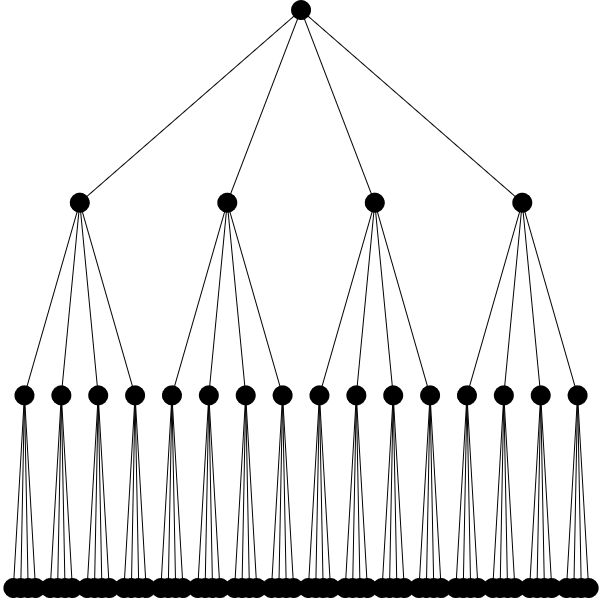
\includegraphics[width=.9\linewidth]{../screenshots/lineargraphexample.PNG}
		\caption{Baumdarstellung in traditioneller Form}
		\label{fig:test1}
	\end{minipage}%
	\begin{minipage}{.5\textwidth}
		\centering
		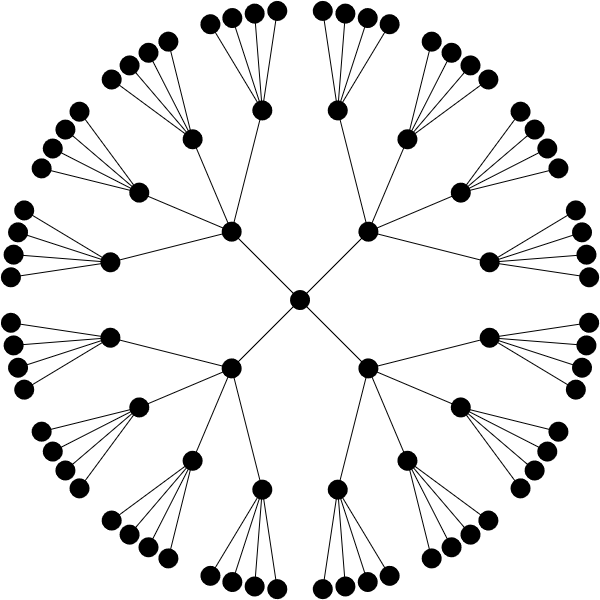
\includegraphics[width=.9\linewidth]{../screenshots/radialgraphexample.PNG}
		\caption{Kreisförmige Baumdarstellung}
		\label{fig:test2}
	\end{minipage}
\end{figure}
\todo{Bild+Argumentation einfügen zur Platzersparnis durch kreisförmige Anordnung}
D3 bietet zur Berechnung einer sinnvollen Knotenanordnung von Bäumen die Funktion $d3.tree()$ an, welche allen Knoten eines Baumes x- und y-Koordinaten jeweils im Bereich von 0 bis 1 zuordnet. Es liegt dann in der Hand des Programmierers, diese sinnvoll zu interpretieren. Um die Knoten, wie in der Abbildung gezeigt in konzentrischen Kreisen anzuordnen eignen sich Polarkoordinaten ausgezeichnet. Die y-Koordinate wird als Radius $\rho$, die x-Koordinate als Polarwinkel $\varphi$ interpretiert.
\begin{align}
&\rho = y\\
&\varphi = 2 \cdot \pi \cdot x
\end{align}
Zur Darstellung auf dem Bildschirm müssen $\rho$ und $\varphi$ anschließend in kartesische Koordinaten $x_{screen}$ und $y_{screen}$ umgerechnet werden. Die allgemeinen Umrechnungsformeln ergeben sich als
\begin{align}
&x_{screen} = \rho \cdot \cos (\varphi)\\
&y_{screen} = \rho \cdot \sin (\varphi)
\end{align}
Bei dieser Umrechnung wird allerdings noch nicht berücksichtigt, dass die gegebenen Polarkoordinaten auf generischen Koordinaten im Bereich $[0,1]$ basieren. Zur korrekten Positionierung müssen noch eine Skalierung auf die verfügbare Breite (width) $w$ und Höhe (height) $h$, sowie eine Verschiebung in die Mitte der Anzeige vorgenommen werden. Es entstehen die endgültigen Formeln
\begin{align}
&x_{screen} = \rho \cdot \cos (\varphi) \cdot w + \frac{w}{2}\\
&y_{screen} = \rho \cdot \sin (\varphi) \cdot h + \frac{h}{2}
\end{align}